% ============================================================
\section{Desarrollo y Metodología}
% ============================================================

\subsection{Entorno Experimental}

Los experimentos se ejecutaron en dos entornos de hardware complementarios: el
entrenamiento del caso A se realizó en Google Colab (GPU Tesla T4), mientras
que los casos B y C se ejecutaron en una estación del laboratorio de Cómputo~8
(espacio de trabajo \texttt{\char`\~/paul} en el equipo
\texttt{cisco-optiplex7000}). La Tabla~\ref{tab:hardware} resume ambas
plataformas según lo reportado por \texttt{lscpu}, \texttt{free -h} y
\texttt{nvidia-smi}.

\begin{table}[H]
\centering
\caption{Entornos de hardware utilizados en el benchmark.}
\label{tab:hardware}
\setlength{\tabcolsep}{6pt}
\begin{tabular}{lcc}
  \toprule
  \textbf{Componente} & \textbf{Google Colab (Caso A)} & \textbf{Laboratorio (Casos B y C)} \\
  \midrule
  CPU              & Intel Xeon @ 2.20\,GHz (2 vCPU) & Intel Core i9-12900K (24 hilos) \\
  RAM              & 12.7\,GiB                        & 31\,GiB \\
  GPU              & NVIDIA Tesla T4                  & NVIDIA GeForce RTX 3070 \\
  VRAM             & 15\,360\,MiB                     & 8\,192\,MiB \\
  Driver / CUDA    & 580.82.07 / CUDA 13.0            & 535.274.02 / CUDA 12.2 \\
  Framework        & PyTorch 2.11.0+cu128             & PyTorch + OpenCV (WITH\_CUDA=ON) \\
  \bottomrule
\end{tabular}
\end{table}

La estación del laboratorio queda identificada de forma unívoca por su interfaz
de red \texttt{enp0s31f6}, con dirección MAC \texttt{08:92:04:e5:9d:24} y
dirección IP \texttt{172.16.12.194}, según la salida de \texttt{ip link}
mostrada en la Figura~\ref{fig:mac}.

\begin{figure}[H]
  \centering
  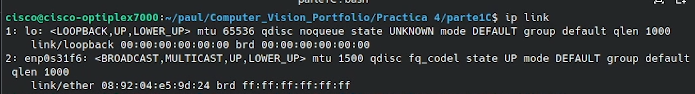
\includegraphics[width=0.95\textwidth]{imagenes/direccion_mac.png}
  \caption{Identificación de la estación de laboratorio mediante \texttt{ip link}:
           interfaz \texttt{enp0s31f6}, MAC \texttt{08:92:04:e5:9d:24}, dentro del
           espacio de trabajo \texttt{\char`\~/paul}.}
  \label{fig:mac}
\end{figure}

La metodología de medición fue uniforme en los tres casos: (i) cada
configuración CPU/GPU se ejecuta como proceso independiente para no contaminar
las mediciones; (ii) el tiempo por cuadro se mide con relojes monotónicos
(\texttt{std::chrono} en C++, \texttt{time.perf\_counter} en Python) y, cuando
interviene CUDA, se sincroniza el dispositivo antes y después de cronometrar
(\texttt{torch.cuda.synchronize()}) para no medir lanzamientos asíncronos;
(iii) el estado del sistema se monitorea en paralelo con \texttt{btop},
\texttt{top}, \texttt{ps} y \texttt{nvidia-smi}.

% ------------------------------------------------------------
\subsection{Caso A: Fine-Tuning de YOLO26n-seg}
\label{sec:casoA}

Se realizó el ajuste fino del modelo preentrenado \texttt{yolo26n-seg.pt}
(Ultralytics \cite{Ultralytics}) sobre el conjunto de datos propio
\textit{Tools segmentation}, etiquetado y exportado desde
Roboflow\footnote{\url{https://app.roboflow.com/paul-space-qcfcl/tools-segmentation-f2nhg-tf2cd/1}}:
3\,097 imágenes de herramientas (martillo, alicate,
tornillo, llave) divididas en 2\,709 de entrenamiento y 388 de prueba; la
validación se realizó sobre 406 imágenes con 772 instancias. El entrenamiento
se configuró con 60 épocas, resolución de entrada de $640\times640$, lote de 16
y paciencia de 15 épocas.

La sesión de Colab confirmó la disponibilidad del dispositivo CUDA antes de
entrenar: la Figura~\ref{fig:cuda_colab} muestra PyTorch 2.11.0+cu128 con
\texttt{CUDA disponible: True} y la Tesla T4 en reposo (3\,MiB de VRAM, 11\,W,
0\,\% de utilización) según \texttt{nvidia-smi}.

\begin{figure}[H]
  \centering
  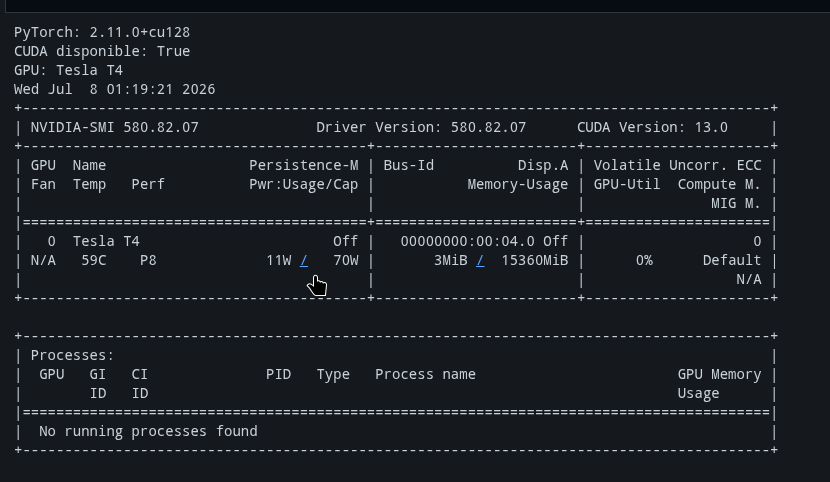
\includegraphics[width=0.85\textwidth]{imagenes/sectionA/cuda_disponible.png}
  \caption{Verificación del entorno en Google Colab: PyTorch 2.11.0+cu128,
           CUDA 13.0 y GPU Tesla T4 (15\,360\,MiB de VRAM) en estado de reposo.}
  \label{fig:cuda_colab}
\end{figure}

Del registro de entrenamiento se extraen la primera y la última época, que
evidencian la evolución del aprendizaje:

\begin{lstlisting}[style=code]
Epoch  GPU_mem  box_loss  seg_loss  cls_loss  dfl_loss   Instances  Size
 1/60    3.31G    0.8241     1.925     4.503  0.009851         67   640
        all  406  772  Box(P 0.539  R 0.189  mAP50 0.192  mAP50-95 0.137)
                       Mask(P 0.507  R 0.161  mAP50 0.151  mAP50-95 0.069)

60/60     4.6G    0.5509    0.7458    0.4008  0.009804         20   640
        all  406  772  Box(P 0.897  R 0.691  mAP50 0.792  mAP50-95 0.695)
                       Mask(P 0.898  R 0.692  mAP50 0.792  mAP50-95 0.606)
\end{lstlisting}

Entre la época 1 y la 60 la pérdida de clasificación cae de 4.503 a 0.4008
(un orden de magnitud) y la de segmentación de 1.925 a 0.7458, mientras el
mAP50 de cajas sube de 0.192 a 0.792. El consumo de VRAM se mantuvo estable
entre 3.31 y 4.6\,GiB de los 15\,GiB disponibles en la T4. Cada época tomó en
promedio 1\,min\,30\,s (144 lotes a 1.6--2.6\,it/s más la validación), lo que
arroja un total aproximado de \textbf{90 minutos de entrenamiento en GPU}. El
mismo entrenamiento lanzado sobre la CPU del entorno Colab (Xeon de 2 vCPU)
tomó entre 3.5 y 4 horas, con el kernel de Python saturando el procesador de
forma sostenida: \texttt{top} y \texttt{ps aux --sort=-\%cpu} registraron al
proceso \texttt{python3} en 87--100\,\% de CPU y hasta 5.2\,GiB de RAM
residente (41\,\% de la memoria del entorno), como se aprecia en el siguiente
extracto de monitoreo:

\begin{lstlisting}[style=code]
top - 17:12:08  load average: 1.33, 1.25, 0.82
%Cpu(s): 34.6 us, 18.6 sy, 45.8 id
MiB Mem : 12975.5 total, 3081.2 free, 6269.7 used

  PID USER  PR NI    VIRT    RES   SHR S  %CPU %MEM  COMMAND
 1931 root  20  0 7137180   5.2g 169120 R 100.0 41.2 python3 -m colab_kernel_lau
\end{lstlisting}

Las métricas finales de validación del modelo ajustado fueron
mAP50 $= 0.791$ y mAP50-95 $= 0.693$ para cajas, y mAP50 $= 0.790$ con
mAP50-95 $= 0.604$ para máscaras.

Posteriormente, los pesos entrenados se descargaron y se evaluaron en
inferencia local sobre CPU: predicción de imágenes estáticas del conjunto de
demostración y clasificación en vivo desde la cámara web, alcanzando alrededor
de \textbf{10.9 FPS} en tiempo real (Sección~\ref{sec:res_a}).

% ------------------------------------------------------------
\subsection{Caso B: Inferencia YOLOv12n vs.\ YOLO26n y Real-ESRGAN}
\label{sec:casoB}

El segundo caso compara, sobre la estación del laboratorio (i9-12900K +
RTX 3070), el rendimiento de inferencia de dos variantes ligeras de la familia
YOLO ---\texttt{yolo12n.pt} y \texttt{yolo26n.pt}--- ejecutadas sobre el mismo
video de prueba (\texttt{personas.mp4}) en cuatro combinaciones:
$\{$YOLOv12n, YOLO26n$\} \times \{$\texttt{cpu}, \texttt{cuda}$\}$. Cada
corrida superpone en pantalla el FPS instantáneo mientras \texttt{btop}
registra el estado de los 24 hilos de la CPU, la RAM y la GPU.

Como carga complementaria de cómputo intensivo se evaluó la red de
superresolución \textbf{Real-ESRGAN x4plus} (RRDBNet de 23 bloques residuales)
\cite{Wang2021} sobre un video en dos modalidades: procesamiento continuo de un
recorte central de $160\times160$\,px (ampliado $\times4$), y muestreo de un
cuadro completo cada 2 segundos. En la primera modalidad se registró el FPS en
vivo; en la segunda, el tiempo de procesamiento por cuadro: 1.12\,s en GPU
frente a 4.40\,s en CPU.

% ------------------------------------------------------------
\subsection{Caso C: Detección de Bordes en C++ (OpenCV / CUDA)}
\label{sec:casoC}

El tercer caso implementa en C++ un pipeline clásico de preprocesamiento sobre
video: conversión a escala de grises $\to$ suavizado gaussiano ($5\times5$,
$\sigma=1.5$) $\to$ erosión $\to$ dilatación $\to$ detección de bordes de Canny
(umbrales 50/150) \cite{Canny1986} en paralelo con ecualización de histograma.
Se compilaron \textbf{dos ejecutables independientes} a partir de dos archivos
fuente principales:

\begin{itemize}
  \item \texttt{src/pipeline\_cpu.cpp} $\to$ \texttt{preprocesamiento\_cpu}:
        toda la cadena sobre \texttt{cv::Mat}; compila con cualquier OpenCV.
  \item \texttt{src/pipeline\_gpu.cpp} $\to$ \texttt{preprocesamiento\_gpu}:
        la misma cadena sobre \texttt{cv::cuda::GpuMat}, con \emph{una única
        subida} (\texttt{upload}) del cuadro a VRAM y \emph{una única bajada}
        (\texttt{download}) del resultado, manteniendo todos los pasos
        intermedios en memoria de video. Requiere OpenCV compilado con
        \texttt{WITH\_CUDA=ON}, disponible como instalación de sistema en el
        laboratorio.
\end{itemize}

Separar ambas mediciones en programas distintos evita mezclar contadores de
tiempo en un mismo bucle. Cada ejecutable calcula un promedio móvil de 60
cuadros del tiempo de procesamiento y lo superpone en pantalla junto al FPS
equivalente; los filtros CUDA (gaussiano, morfológicos y Canny) se crean una
sola vez fuera del bucle para no recompilar el kernel en cada cuadro. Durante
la ejecución, el sistema se monitoreó con \texttt{btop} y \texttt{nvidia-smi}
(Sección~\ref{sec:res_c}).
